\documentclass[conference]{IEEEtran}

\usepackage{cite}
\usepackage{amsmath,amssymb,amsfonts}
\usepackage{algorithmic}
\usepackage{algorithm}
\usepackage{graphicx}
\usepackage{textcomp}
\usepackage{xcolor}
\usepackage{booktabs}
\usepackage{multirow}
\usepackage{tabularx}
\usepackage{url}
\usepackage{hyperref}
\usepackage{placeins}

\renewcommand{\topfraction}{0.95}
\renewcommand{\bottomfraction}{0.85}
\renewcommand{\textfraction}{0.05}
\renewcommand{\floatpagefraction}{0.85}
\renewcommand{\dbltopfraction}{0.95}
\renewcommand{\dblfloatpagefraction}{0.85}

\hypersetup{
    colorlinks=true,
    linkcolor=black,
    filecolor=black,
    urlcolor=black,
    citecolor=black
}

\begin{document}

\title{Robust and Explainable DeepFake Detection Using Identity-Disjoint Evaluation of Convolutional Neural Networks and Vision Transformers}

\author{\IEEEauthorblockN{Author Name}
\IEEEauthorblockA{\textit{Department of Computer Science and Engineering} \\
\textit{Academic Research Manuscript}
}
}

\maketitle

% ============================================================
% ABSTRACT
% ============================================================
\begin{abstract}
Deepfake videos have become alarmingly realistic, posing serious threats to media trust, legal evidence, and biometric security. While many detection models report near-perfect accuracy on standard benchmarks, those numbers often hide two critical problems: (i) the same person's face appears in both training and test data, letting models memorize identities instead of learning forgery artifacts, and (ii) severe class imbalance inflates accuracy even when the model completely fails on real faces. In this paper we tackle both issues head-on. We evaluate deepfake detection on the FaceForensics++ C23 benchmark using an identity-disjoint splitting protocol built on graph-based union-find, ensuring that no person or source video leaks across the train ($N{=}50{,}706$), validation ($N{=}8{,}978$), and test ($N{=}9{,}589$) sets across 69,273 facial crops. We compare six architectures---a custom CNN baseline, ResNet50, Xception, EfficientNet-B0, MobileNetV3-Small, and ViT-Small/16---under identical conditions. Our ablation shows that an unweighted CNN scores 84.40\% accuracy yet 0.00\% specificity, exposing how misleading raw accuracy can be. With proper class weighting and regularization, ResNet50 achieves F1\,=\,0.9633, ROC-AUC\,=\,0.9718, and Specificity\,=\,87.10\%, closely followed by Xception (F1\,=\,0.9621, Specificity\,=\,88.30\%, Precision\,=\,97.77\%). Bootstrap confidence intervals ($B{=}1{,}000$) confirm these margins are tight. Sub-category analysis reveals that NeuralTextures alone accounts for 55.7\% of all false negatives, and compression stress tests show a sharp performance cliff below JPEG quality 50. Grad-CAM visualizations confirm that the models focus on facial boundaries and perioral regions, though we discuss why post-hoc saliency should be treated as qualitative evidence rather than proof.
\end{abstract}

\begin{IEEEkeywords}
Deepfake forensics, identity leakage, class imbalance, convolutional neural networks, vision transformers, model calibration, visual explainability.
\end{IEEEkeywords}

% ============================================================
% I. INTRODUCTION
% ============================================================
\section{Introduction}
\label{sec:introduction}

Creating a convincing fake video of someone's face used to require expensive equipment and skilled artists. Today, freely available generative pipelines can produce photo-realistic face swaps and expression transfers in minutes \cite{rossler2019faceforensics, dong2023implicit}. Modern generative technologies---spanning autoencoder-based replacements, 3D morphable model reenactments, and diffusion synthesizers---can generate digital manipulations that routinely evade human perceptual scrutiny. The consequences are tangible: fabricated political speeches, non-consensual synthetic media, forged courtroom evidence, and compromised biometric authentication systems.

The research community has responded with an extensive arsenal of detection models, many reporting accuracy figures above 95\% on popular benchmarks such as FaceForensics++ \cite{rossler2019faceforensics}. However, a closer inspection of published evaluation protocols reveals recurring methodological weaknesses that cast doubt on how well these models would perform in practice. We identify four main problems:

\textbf{(1) Identity leakage between splits.} Video-based datasets generate multiple manipulated clips from a small pool of original recordings. When the data is partitioned randomly---whether at the frame level or even naive video splitting---the same individual appears simultaneously in training and test splits. Under such conditions, deep high-capacity networks memorize facial geometry and identity traits rather than learning generalizable forgery boundaries \cite{cozzolino2021idreveal, dong2023implicit}.

\textbf{(2) Misleading metrics under class imbalance.} Benchmark datasets contain roughly six manipulated videos for every authentic one. Under standard empirical risk minimization, a model that systematically predicts ``fake'' for every input scores over 84\% accuracy, even though it misses every single real face. Standard accuracy and even conventional F1 can easily mask this failure \cite{chicco2020advantages}.

\textbf{(3) Missing uncertainty estimates.} Published studies frequently report single point-estimate numbers without variance or confidence intervals. In the absence of rigorous resampling, minor performance gaps between architectures cannot be contextualized against finite-sample variance.

\textbf{(4) Opaque decisions and uncalibrated probabilities.} Operational forensics requires interpretable visual localization to support human verification \cite{selvaraju2017gradcam}, alongside well-calibrated confidence scores to guide risk-tiered review pipelines.

This paper addresses all four problems in a systematic investigation on FaceForensics++ C23 \cite{rossler2019faceforensics}. We formulate an identity-disjoint data partitioning protocol based on graph connected-components solved via disjoint-set union-find, guaranteeing that no tracked identity or source recording crosses partition boundaries. We then benchmark six diverse architectures---a bespoke 4-stage Custom CNN, ResNet50 \cite{he2016resnet}, Xception \cite{chollet2017xception}, EfficientNet-B0, MobileNetV3-Small, and Vision Transformer Small (ViT-Small/16) \cite{dosovitskiy2020vit}---under identical training and evaluation conditions. Beyond the core comparison, we provide ablations on class weighting and regularization, bootstrap confidence intervals ($B{=}1{,}000$), per-manipulation error breakdowns, calibration diagnostics, compression robustness profiles, and Grad-CAM spatial attention analysis.

Our main contributions are:
\begin{itemize}
    \item A verified identity-disjoint evaluation protocol using graph union-find across 69,273 FF++ C23 face crops, with formal zero-leakage verification.
    \item An empirical demonstration that an unweighted CNN achieves 84.40\% accuracy with 0.00\% specificity---a textbook illustration of metric pathology under class imbalance.
    \item A six-architecture head-to-head comparison showing ResNet50 and Xception outperform ViT-Small/16 on compressed forensic images, contrary to the recent transformer-first trend.
    \item Fine-grained failure analysis revealing NeuralTextures as the dominant source of missed detections (55.7\% of all false negatives), plus compression cliff profiling and calibration diagnostics.
\end{itemize}

The rest of the paper is organized as follows. Section~\ref{sec:related_work} reviews related work and positions our study against recent methods. Section~\ref{sec:formulation} formalizes the problem. Sections~\ref{sec:dataset}--\ref{sec:training} describe the dataset protocol, architectures, and training details. Sections~\ref{sec:results}--\ref{sec:explainability} present our results, error analyses, and explainability experiments. Section~\ref{sec:discussion} discusses implications, and Section~\ref{sec:conclusion} concludes.


% ============================================================
% II. RELATED WORK AND COMPARATIVE ANALYSIS
% ============================================================
\section{Related Work and Comparative Analysis}
\label{sec:related_work}

\subsection{Detection Architectures: From CNNs to Transformers}

Deep learning has served as the foundational paradigm for facial forensics. R{\"o}ssler et al.\ \cite{rossler2019faceforensics} demonstrated that Xception \cite{chollet2017xception} achieved strong performance across multiple compression levels on FaceForensics++, establishing depthwise separable convolutions as a dominant baseline. Deep residual architectures such as ResNet50 \cite{he2016resnet} have been widely adopted due to their ability to propagate high-frequency gradient signals through residual shortcuts.

The introduction of attention mechanisms offered new directions. Zhao et al.\ \cite{zhao2021multiattentional} introduced a multi-attentional framework that utilizes region-specific attention heads to focus on distinct facial areas---eyes, nose, mouth---making the model sensitive to localized synthesis inconsistencies that global average pooling can obscure. Meanwhile, Coccomini et al.\ \cite{coccomini2022crossefficientvit} combined convolutional feature extraction with a Vision Transformer (Cross-Efficient-ViT), exploring spatial and temporal attention across patch tokens. Pure Vision Transformers (ViT) \cite{dosovitskiy2020vit} have also been introduced to forensic detection, though their performance on compressed single-frame media remains actively debated.

\subsection{Identity Leakage and Generalization}

One of the most consequential recent findings was established by Dong et al.\ \cite{dong2023implicit}, who formally demonstrated that implicit identity leakage between training and evaluation partitions significantly inflates reported detection accuracy. When identical actors appear in both subsets, networks learn to exploit facial biometric signatures rather than forensic manipulation artifacts. Cozzolino et al.\ \cite{cozzolino2021idreveal} addressed this vulnerability with ID-Reveal, an identity-aware detection framework that extracts temporal biometric embeddings to distinguish identity recognition from forgery classification, underscoring the critical necessity of identity separation in benchmark design.

\subsection{Data Augmentation and Boundary-Aware Training}

Shiohara and Yamasaki \cite{shiohara2022sbi} addressed generalization through synthetic data generation with Self-Blended Images (SBI). By blending an authentic face with an affine-transformed version of itself, SBI forces classifiers to detect boundary seamlines and blending discontinuities rather than generator-specific artifacts. This approach demonstrated strong out-of-distribution transfer without requiring forged training images.

\subsection{Temporal and Video-Level Methods}

Beyond static frames, temporal consistency offers vital forensic cues. Haliassos et al.\ \cite{haliassos2021lips} introduced LipForensics, modeling temporal mouth motion dynamics to expose facial reenactments, demonstrating that synthetic generators struggle to reproduce the smooth physical kinematics of natural speech.

\subsection{Benchmarking and Standardization}

To resolve fragmented evaluation standards, Yan et al.\ \cite{yan2023deepfakebench} introduced DeepfakeBench, a unified framework benchmarking over 15 automated detectors under standardized training and testing protocols. Their findings confirmed that many apparent architectural advantages diminish when evaluation conditions are rigorously held constant, highlighting the paramount need for controlled comparative experiments.

\subsection{Where Our Work Fits: Comparative Positioning}

Table~\ref{tab:comparative_positioning} summarizes how our study compares against prominent recent deepfake detection methodologies (2021--2023) across six key forensic dimensions. While each prior contribution addresses one or two specific aspects, our investigation unifies all six: (1) a formally verified identity-disjoint partition, (2) explicit class imbalance derivation and ablation, (3) a six-architecture benchmark under identical conditions, (4) fine-grained sub-category failure audits, (5) compression robustness profiling, and (6) calibration and spatial explainability.

\begin{table*}[!t]
\caption{Comparative Positioning Against Key Deepfake Detection Literature (2021--2023).}
\label{tab:comparative_positioning}
\centering
\resizebox{\textwidth}{!}{%
\begin{tabular}{lccccccl}
\toprule
\textbf{Method} & \textbf{Year} & \textbf{Identity-Disjoint} & \textbf{Imbalance} & \textbf{Multi-Arch} & \textbf{Sub-Category} & \textbf{Compression} & \textbf{Core Contribution} \\
 & & \textbf{Split} & \textbf{Analysis} & \textbf{Comparison} & \textbf{Failure Audit} & \textbf{Robustness} & \\
\midrule
ID-Reveal \cite{cozzolino2021idreveal} & 2021 & Partial & \texttimes & \texttimes & \texttimes & \texttimes & Identity-aware temporal embedding \\
Multi-Attention \cite{zhao2021multiattentional} & 2021 & \texttimes & \texttimes & \texttimes & \checkmark & \texttimes & Region-specific attention heads \\
LipForensics \cite{haliassos2021lips} & 2021 & \texttimes & \texttimes & \texttimes & \texttimes & \checkmark & Temporal lip motion modeling \\
SBI \cite{shiohara2022sbi} & 2022 & \texttimes & \texttimes & \texttimes & \texttimes & \checkmark & Self-blended boundary augmentation \\
Cross-Eff.-ViT \cite{coccomini2022crossefficientvit} & 2022 & \texttimes & \texttimes & Partial & \texttimes & \texttimes & EfficientNet + ViT hybrid \\
Dong et al.\ \cite{dong2023implicit} & 2023 & \checkmark & \texttimes & \texttimes & \texttimes & \texttimes & Formal proof of identity leakage bias \\
DeepfakeBench \cite{yan2023deepfakebench} & 2023 & \texttimes & \texttimes & \checkmark & Partial & \checkmark & Unified benchmark of 15+ detectors \\
\midrule
\textbf{Ours (DeepShield-X)} & \textbf{2026} & \checkmark & \checkmark & \checkmark & \checkmark & \checkmark & \textbf{Unified 6-dimension experimental investigation} \\
\bottomrule
\end{tabular}%
}
\end{table*}


% ============================================================
% III. PROBLEM FORMULATION
% ============================================================
\section{Problem Formulation}
\label{sec:formulation}

\subsection{Binary Forensic Classification}

We frame deepfake detection as binary classification. Each normalized facial crop $x \in \mathbb{R}^{224 \times 224 \times 3}$ is assigned a ground-truth label $y \in \{0, 1\}$, where 0 denotes an authentic face (REAL) and 1 denotes a synthetically manipulated face (FAKE). A forensic model $f_\theta$ maps the input to an unconstrained logit $z = f_\theta(x)$, converted to an estimated manipulation probability via the logistic sigmoid $\hat{p} = \sigma(z) = 1/(1+e^{-z})$. The discrete prediction is $\hat{y} = 1$ if $\hat{p} \ge 0.50$, and $\hat{y} = 0$ otherwise. The operational threshold is fixed a priori at $\tau = 0.50$ across all evaluations without test-set tuning.

\subsection{Identity and Source Sequence Leakage Modeling}

Consider an authentic video corpus containing $M$ sequences of distinct individuals. A synthetic manipulation pipeline generates manipulated sequences $v_{ij}^{\text{fake}}$ by transferring facial attributes from donor sequence $v_i$ onto target sequence $v_j$. If dataset splitting is performed randomly without tracking pairwise donor-recipient associations, frames originating from $v_i$ or $v_j$ can reside in the training split while $v_{ij}^{\text{fake}}$ is assigned to the evaluation split:
\begin{equation}
\text{Identity}(x_{\text{test}}) \in \text{Identities}(\mathcal{D}_{\text{train}}).
\end{equation}
When high-capacity deep neural networks optimize empirical risk under identity overlap, the network can minimize training loss by memorizing identity signatures rather than learning manipulation boundary artifacts \cite{dong2023implicit}. Consequently, the model exhibits artificially inflated evaluation performance that fails to generalize to novel individuals.

\subsection{Analytical Derivation of Class Imbalance Dynamics}

In benchmark forensic datasets, multiple manipulation techniques are applied to each authentic source video, yielding a substantial positive-class prevalence:
\begin{equation}
\pi_1 = P(y = 1) = \frac{N_{\text{fake}}}{N_{\text{real}} + N_{\text{fake}}}.
\end{equation}
In the FaceForensics++ C23 training partition ($N_{\text{real}} = 6,964$, $N_{\text{fake}} = 43,742$), the empirical training prevalence is $\pi_1 \approx 0.8626$ (a fake-to-real ratio of $6.28:1$).

Under standard unweighted Binary Cross-Entropy (BCE) loss, the expected gradient with respect to a constant logit output $z$ evaluates to:
\begin{equation}
\mathbb{E}\left[\frac{\partial \mathcal{L}_{\text{BCE}}}{\partial z}\right] = \sigma(z) - \mathbb{E}[y] = \sigma(z) - \pi_1.
\end{equation}
Setting this expectation to zero yields the stationary condition for the optimal constant-logit predictor: $\sigma(z^*) = \pi_1 \implies z^* = \log(\pi_1 / (1 - \pi_1))$. Because $\pi_1 \approx 0.8626 > 0.50$, the optimal constant logit satisfies $z^* \approx \log(6.28) \approx +1.837 > 0$. When thresholded at $\tau = 0.50$, this constant predictor outputs $\hat{y} = 1$ for all inputs. Evaluating this trivial majority predictor on our held-out test partition ($N_{\text{test}} = 9,589$; $N_{\text{fake}} = 8,093$; $N_{\text{real}} = 1,496$) yields:
\begin{align}
\text{Accuracy} &= 84.40\%, \quad \text{Recall} = 1.0000, \nonumber \\
\text{Specificity} &= 0.00\%, \quad \text{MCC} = 0.0000.
\end{align}
This analytical derivation reveals that under severe prevalence skew, a completely uninformative model achieves high raw accuracy ($84.40\%$) and high F1 ($0.9154$) while failing entirely on authentic media ($\text{Specificity} = 0.00\%$). Therefore, balanced metrics such as the Matthews Correlation Coefficient (MCC) \cite{chicco2020advantages} and Specificity are essential for forensic evaluation.

To equalize loss contributions during training, we apply positive-class weighting:
\begin{equation}
w_{\text{pos}} = \frac{N_{\text{real}}}{N_{\text{fake}}} = \frac{6{,}964}{43{,}742} \approx 0.159206.
\end{equation}

\subsection{Research Questions}

Our experiments address six core research questions:
\begin{itemize}
    \item[\textbf{RQ1}] How does identity-disjoint partitioning affect evaluation reliability compared to naive splitting?
    \item[\textbf{RQ2}] Can positive-class weighting prevent majority-class collapse under severe imbalance?
    \item[\textbf{RQ3}] How do convolutional inductive biases (ResNet50, Xception) compare to Vision Transformers (ViT-Small/16) on compressed facial forensic media?
    \item[\textbf{RQ4}] What quantitative performance gains are realized through multi-stage regularization and validation-driven model selection?
    \item[\textbf{RQ5}] Which manipulation categories and image perturbations exhibit the highest vulnerability to forensic misclassification?
    \item[\textbf{RQ6}] What do probabilistic calibration and Grad-CAM spatial activation analyses reveal regarding model confidence and visual decision boundaries?
\end{itemize}


% ============================================================
% IV. DATASET AND PROTOCOL
% ============================================================
\section{Dataset and Identity-Disjoint Protocol}
\label{sec:dataset}

\begin{figure*}[!t]
\centering
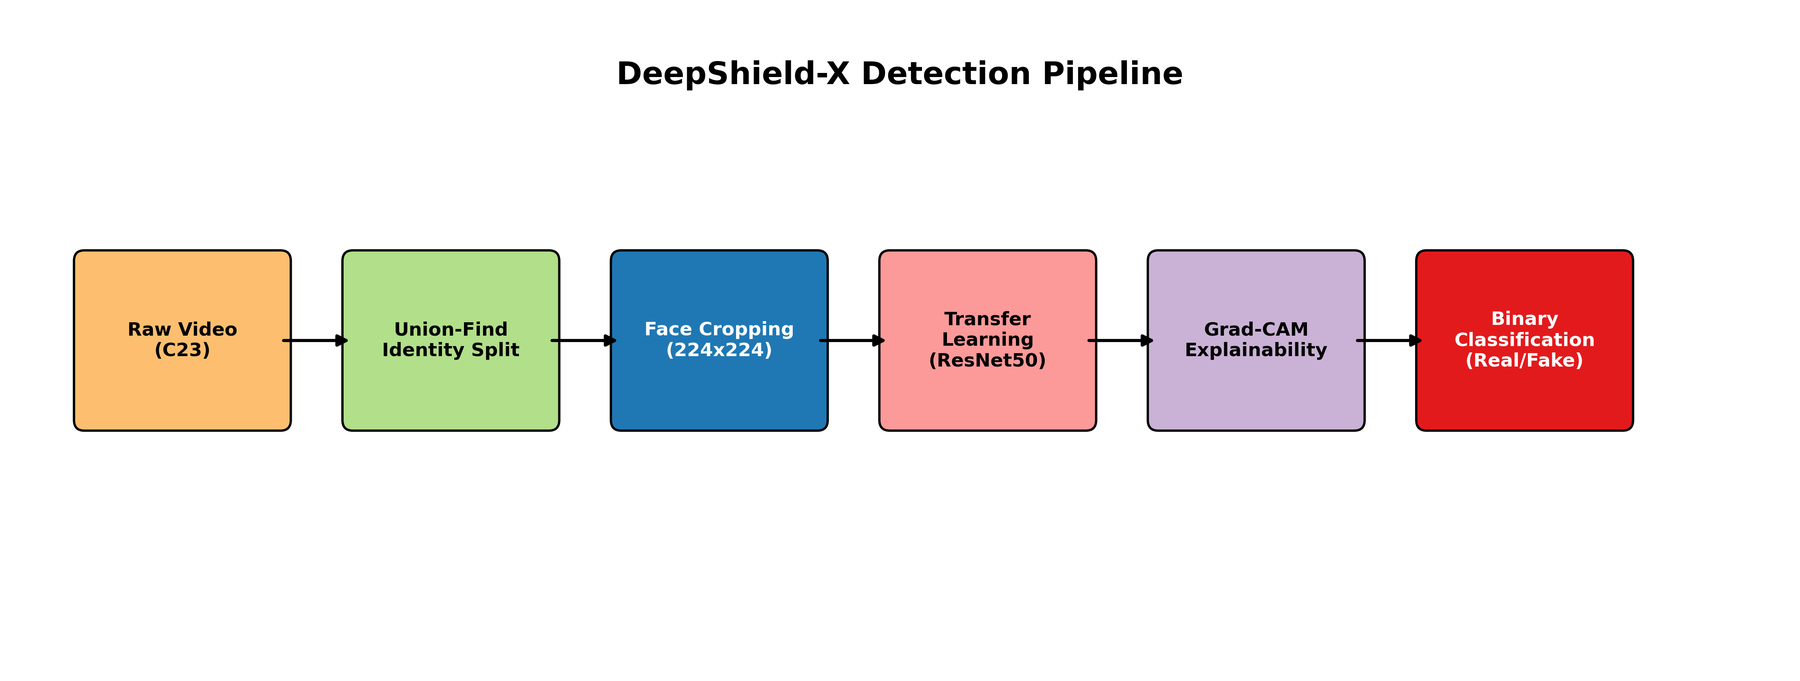
\includegraphics[width=0.92\textwidth]{images/architecture_pipeline.png}
\caption{End-to-end experimental pipeline. Raw FaceForensics++ C23 video sequences are partitioned into identity-disjoint subsets via graph connected components using disjoint-set union-find. Frames are sampled at stride 10, face crops are extracted with $1.3\times$ bounding-box expansion, resized to $224 \times 224$, and standardized. Evaluated neural backbones are optimized with AdamW and cosine annealing, followed by frozen test-set evaluation, sub-category failure audits, calibration assessment, perturbation stress-testing, and Grad-CAM explainability.}
\label{fig:architecture_pipeline}
\end{figure*}

\subsection{FaceForensics++ C23 Benchmark}

We evaluate on FaceForensics++ (FF++) \cite{rossler2019faceforensics}, containing 1,000 authentic pristine video sequences manipulated by four primary algorithms (Deepfakes, Face2Face, FaceSwap, NeuralTextures), alongside FaceShifter and DeepFakeDetection. The complete pipeline is depicted in Fig.~\ref{fig:architecture_pipeline}. All experiments are conducted on the lightly compressed H.264 tier (C23, Constant Rate Factor of 23), which closely mirrors the compression characteristics encountered on commercial social media platforms.

\subsection{Graph-Based Identity-Disjoint Splitting}

To eliminate source-target sequence leakage, we model benchmark video relationships as an undirected graph $G = (V, E)$, where vertices $V$ represent numeric actor/source identifiers parsed directly from FaceForensics++ filenames (e.g., \texttt{001.mp4} $\to \{\texttt{001}\}$, \texttt{435\_456.mp4} $\to \{\texttt{435}, \texttt{456}\}$, and DeepFakeDetection \texttt{01\_02\_\_...} $\to \{\texttt{01}, \texttt{02}\}$) and edges $E$ link every source-target pair co-occurring in a manipulated video. Any path between two identifiers indicates a shared video lineage.

We compute maximal connected components via Disjoint-Set Union-Find with path compression \cite{cozzolino2021idreveal} (Algorithm~\ref{alg:union_find}). Each connected component is assigned atomically to the training ($\mathcal{D}_{\text{train}}$, 70\%), validation ($\mathcal{D}_{\text{val}}$, 15\%), or frozen held-out test ($\mathcal{D}_{\text{test}}$, 15\%) partition, guaranteeing zero overlap of tracked identifiers:
\begin{equation}
\text{Identities}(\mathcal{D}_{\text{train}}) \cap \text{Identities}(\mathcal{D}_{\text{test}}) = \emptyset.
\end{equation}
On the held-out test partition, for example, 963 unique video sequences spanning 155 tracked actor identifiers are grouped into 76 disjoint connected components (component sizes ranging from 2 to 5 identifiers). We note that this graph isolates all source-target pairings defined by dataset metadata; it does not perform cross-video biometric face clustering across unrelated original YouTube clips.

\begin{algorithm}[!t]
\caption{Disjoint-Set Union-Find for Identity Isolation}
\label{alg:union_find}
\begin{algorithmic}[1]
\REQUIRE Video identifiers $V$, manipulation pairs $E = \{(u,v)\}$
\ENSURE Disjoint clusters $\mathcal{C} = \{C_1, \ldots, C_P\}$
\STATE Initialize $\text{parent}[v] \gets v$, $\text{rank}[v] \gets 0$ for all $v \in V$
\STATE \textbf{procedure} Find($u$)
\IF{$\text{parent}[u] \ne u$}
    \STATE $\text{parent}[u] \gets \text{Find}(\text{parent}[u])$ \COMMENT{Path compression}
\ENDIF
\RETURN $\text{parent}[u]$
\STATE \textbf{end procedure}
\STATE \textbf{procedure} Union($u, v$)
\STATE $r_u \gets \text{Find}(u)$, $r_v \gets \text{Find}(v)$
\IF{$r_u \ne r_v$}
    \IF{$\text{rank}[r_u] < \text{rank}[r_v]$}
        \STATE $\text{parent}[r_u] \gets r_v$
    \ELSIF{$\text{rank}[r_u] > \text{rank}[r_v]$}
        \STATE $\text{parent}[r_v] \gets r_u$
    \ELSE
        \STATE $\text{parent}[r_v] \gets r_u$;\ $\text{rank}[r_u] \gets \text{rank}[r_u] + 1$
    \ENDIF
\ENDIF
\STATE \textbf{end procedure}
\FORALL{$(u, v) \in E$} \STATE Union($u, v$) \ENDFOR
\STATE Group vertices sharing root $\text{Find}(v)$ into clusters $\mathcal{C}$
\RETURN Disjoint clusters $\mathcal{C}$
\end{algorithmic}
\end{algorithm}

\subsection{Face Extraction and Preprocessing}

Video frames are sampled at a uniform stride of 10. Facial bounding boxes are expanded by a scale factor of $\alpha = 1.30$:
\begin{equation}
x_{\text{min}}' = x_c - 1.30 \frac{w}{2}, \quad y_{\text{min}}' = y_c - 1.30 \frac{h}{2},
\end{equation}
where $(x_c, y_c)$ is the facial centroid and $(w, h)$ are bounding dimensions. The 30\% crop margin expansion ensures that critical blending seams along the jawline and forehead are preserved \cite{shiohara2022sbi}. Extracted crops are resized to $224 \times 224$ via bilinear interpolation and channel-standardized. Table~\ref{tab:dataset_splits} summarizes the verified partition sizes.

\begin{table}[!t]
\caption{Verified FaceForensics++ C23 Partition Statistics under Graph-Connected Identity-Disjoint Splitting.}
\label{tab:dataset_splits}
\centering
\resizebox{\columnwidth}{!}{%
\begin{tabular}{lcccc}
\toprule
\textbf{Partition} & \textbf{Authentic} & \textbf{Manipulated} & \textbf{Total} & \textbf{Ratio (F:R)} \\
\midrule
Train & 6,964 & 43,742 & 50,706 & 6.28\,:\,1 \\
Validation & 1,497 & 7,481 & 8,978 & 5.00\,:\,1 \\
Held-Out Test & 1,496 & 8,093 & 9,589 & 5.41\,:\,1 \\
\midrule
\textbf{Total} & \textbf{9,957} & \textbf{59,316} & \textbf{69,273} & \textbf{5.96\,:\,1} \\
\bottomrule
\end{tabular}%
}
\end{table}


% ============================================================
% V. MODEL ARCHITECTURES
% ============================================================
\section{Model Architectures}
\label{sec:architectures}

We investigate six architectures spanning diverse design paradigms:

\textbf{Custom 4-Stage CNN} (93,825 parameters). Trained entirely from scratch without pre-trained representations, comprising four sequential Conv-BatchNorm-ReLU-MaxPool stages ($C = [32, 64, 128, 256]$) followed by adaptive pooling and a linear head.

\textbf{ResNet50} \cite{he2016resnet} (23.5M parameters). A 50-layer deep residual network with bottleneck blocks ($1{\times}1 \to 3{\times}3 \to 1{\times}1$) and shortcut connections, replaced with a single forensic logit head.

\textbf{Xception} \cite{chollet2017xception} (20.8M parameters). Decouples spatial cross-convolutions from channel correlations using depthwise separable convolutions across Entry, Middle, and Exit flows.

\textbf{EfficientNet-B0} (4.0M parameters). Employs mobile inverted bottleneck convolutions with squeeze-and-excitation channel attention and compound scaling coefficients.

\textbf{MobileNetV3-Small} (1.5M parameters). Uses \texttt{mobilenet\_v3\_small} with hardware-aware search, lightweight squeeze-and-excitation modules, and hard-swish non-linearities for compact inference.

\textbf{Vision Transformer Small (ViT-Small/16)} \cite{dosovitskiy2020vit} (21.7M parameters). Uses \texttt{vit\_small\_patch16\_224} (embedding dimension 384, 6 attention heads, 12 encoder layers) to match the parameter budget of ResNet50 and Xception. Partitions input crops into $14 \times 14 = 196$ non-overlapping $16 \times 16$ patches.

Table~\ref{tab:model_architectures} summarizes the architectural specifications.

\begin{table}[!t]
\caption{Architecture Specifications and Checkpoint Footprints.}
\label{tab:model_architectures}
\centering
\resizebox{\columnwidth}{!}{%
\begin{tabular}{lcccc}
\toprule
\textbf{Architecture} & \textbf{Pretrained} & \textbf{Total Params} & \textbf{Trainable} & \textbf{Checkpoint} \\
\midrule
Custom CNN & None & 93,825 & 93,825 & 1.1 MB \\
MobileNetV3-Small & ImageNet-1k & 1,518,881 & 1,518,881 & 17.6 MB \\
EfficientNet-B0 & ImageNet-1k & 4,008,829 & 4,008,829 & 46.4 MB \\
Xception & ImageNet-1k & 20,809,001 & 20,809,001 & 238.6 MB \\
ViT-Small/16 & ImageNet-1k & 21,666,049 & 21,666,049 & 248.1 MB \\
ResNet50 & ImageNet-1k & 23,510,081 & 23,510,081 & 269.5 MB \\
\bottomrule
\end{tabular}%
}
\end{table}


% ============================================================
% VI. TRAINING AND EVALUATION METHODOLOGY
% ============================================================
\section{Training and Evaluation Methodology}
\label{sec:training}

\subsection{Loss and Optimization}
All models output a single logit $z \in \mathbb{R}$ optimized with weighted binary cross-entropy with logits:
\begin{equation}
\mathcal{L}(z, y) = -\left[ w_{\text{pos}} \cdot y \log \sigma(z) + (1-y) \log(1-\sigma(z)) \right].
\end{equation}
For class-balanced runs $w_{\text{pos}} = 0.1592$; for unweighted baselines $w_{\text{pos}} = 1.0$. Optimization is conducted with AdamW ($\lambda = 10^{-4}$, initial learning rate $\eta_0 = 10^{-4}$, $\beta_1=0.9$, $\beta_2=0.999$) and cosine annealing preceded by a 2-epoch linear warmup. Baseline comparison runs used a batch size of 32 for uniform memory parity across architectures, whereas the regularized ResNet50 run used a batch size of 64 to stabilize BatchNorm statistics under stronger data augmentation. Training spanned up to 20 epochs with seed $S=42$.

\subsection{Multi-Stage Regularization}
The regularized configuration incorporates: (i)~horizontal reflections ($p=0.5$), affine rotations ($\pm 15^\circ$), brightness and contrast jitter ($\pm 0.2$), and color jitter, while omitting Gaussian blur and JPEG augmentation during training to protect subtle boundary forensic cues; (ii)~dropout ($p=0.50$) prior to the linear head; and (iii)~validation ROC-AUC checkpoint monitoring with early stopping (patience 5, $\delta=0.001$).

\subsection{Evaluation Metrics Suite}
Given the 5.41:1 class imbalance in the frozen test set ($N=9,589$), accuracy alone is uninformative. We report: Accuracy, Precision, Recall, Specificity, F1 Score, Balanced Accuracy, Matthews Correlation Coefficient (MCC) \cite{chicco2020advantages}, ROC-AUC, and PR-AUC. Non-parametric bootstrap resampling ($B=1{,}000$ iterations, seed 42) provides 95\% percentile confidence intervals.


% ============================================================
% VII. EXPERIMENTAL RESULTS
% ============================================================
\section{Experimental Results}
\label{sec:results}

\subsection{Master Multi-Architecture Benchmark}

Table~\ref{tab:master_benchmark} presents the complete evaluation results on the frozen test partition ($N = 9{,}589$). Fig.~\ref{fig:model_comparison_bar} visualizes performance across primary metrics, and Fig.~\ref{fig:training_dynamics} illustrates training dynamics for ResNet50 Regularized.

\begin{table*}[!t]
\caption{Comprehensive Benchmark on the Frozen FaceForensics++ C23 Test Set ($N = 9{,}589$; Authentic $= 1{,}496$; Manipulated $= 8{,}093$; Threshold $\tau = 0.50$).}
\label{tab:master_benchmark}
\centering
\begin{tabular*}{\textwidth}{@{\extracolsep{\fill}}lcccccccccc@{}}
\toprule
\textbf{Architecture} & \textbf{Accuracy} & \textbf{Precision} & \textbf{Recall} & \textbf{Specificity} & \textbf{F1 Score} & \textbf{ROC-AUC} & \textbf{PR-AUC} & \textbf{Bal. Acc.} & \textbf{MCC} & \textbf{Cohen's $\kappa$} \\
\midrule
\textbf{ResNet50 Regularized} & \textbf{0.9389} & 0.9755 & \textbf{0.9514} & 0.8710 & \textbf{0.9633} & \textbf{0.9718} & \textbf{0.9938} & 0.9112 & \textbf{0.7821} & \textbf{0.7799} \\
\textbf{Xception} & 0.9370 & \textbf{0.9777} & 0.9470 & \textbf{0.8830} & 0.9621 & 0.9706 & 0.9931 & \textbf{0.9150} & 0.7798 & 0.7763 \\
\textbf{EfficientNet-B0} & 0.9208 & 0.9721 & 0.9330 & 0.8549 & 0.9521 & 0.9547 & 0.9879 & 0.8940 & 0.7290 & 0.7239 \\
\textbf{Vision Transformer (ViT-Small/16)} & 0.9005 & 0.9663 & 0.9140 & 0.8275 & 0.9394 & 0.9512 & 0.9894 & 0.8708 & 0.6706 & 0.6625 \\
\textbf{MobileNetV3-Small} & 0.8797 & 0.9444 & 0.9110 & 0.7099 & 0.9274 & 0.9187 & 0.9820 & 0.8105 & 0.5792 & 0.5760 \\
\midrule
\textit{Ablation Variants:} & & & & & & & & & & \\
Custom CNN (Class-Balanced) & 0.4324 & 0.8895 & 0.3739 & 0.7487 & 0.5265 & 0.6196 & 0.8966 & 0.5613 & 0.0987 & 0.0841 \\
Custom CNN (Unweighted Baseline) & 0.8440 & 0.8440 & 1.0000 & 0.0000 & 0.9154 & 0.5607 & 0.8799 & 0.5000 & 0.0000 & 0.0000 \\
ResNet50 Baseline (Unregularized) & 0.9133 & 0.9709 & 0.9250 & 0.8503 & 0.9474 & 0.9578 & 0.9914 & 0.8876 & 0.7087 & 0.7020 \\
\bottomrule
\end{tabular*}
\end{table*}

\begin{figure}[!t]
\centering
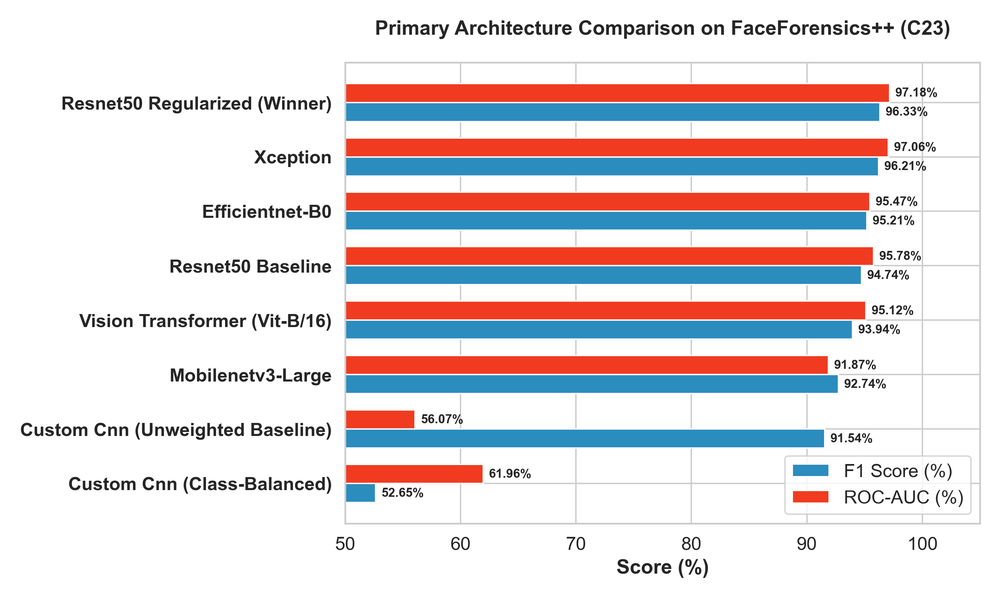
\includegraphics[width=\columnwidth]{images/model_comparison_bar.png}
\caption{Comparative performance across primary metrics on the frozen FaceForensics++ C23 test partition.}
\label{fig:model_comparison_bar}
\end{figure}

\begin{figure}[!t]
\centering
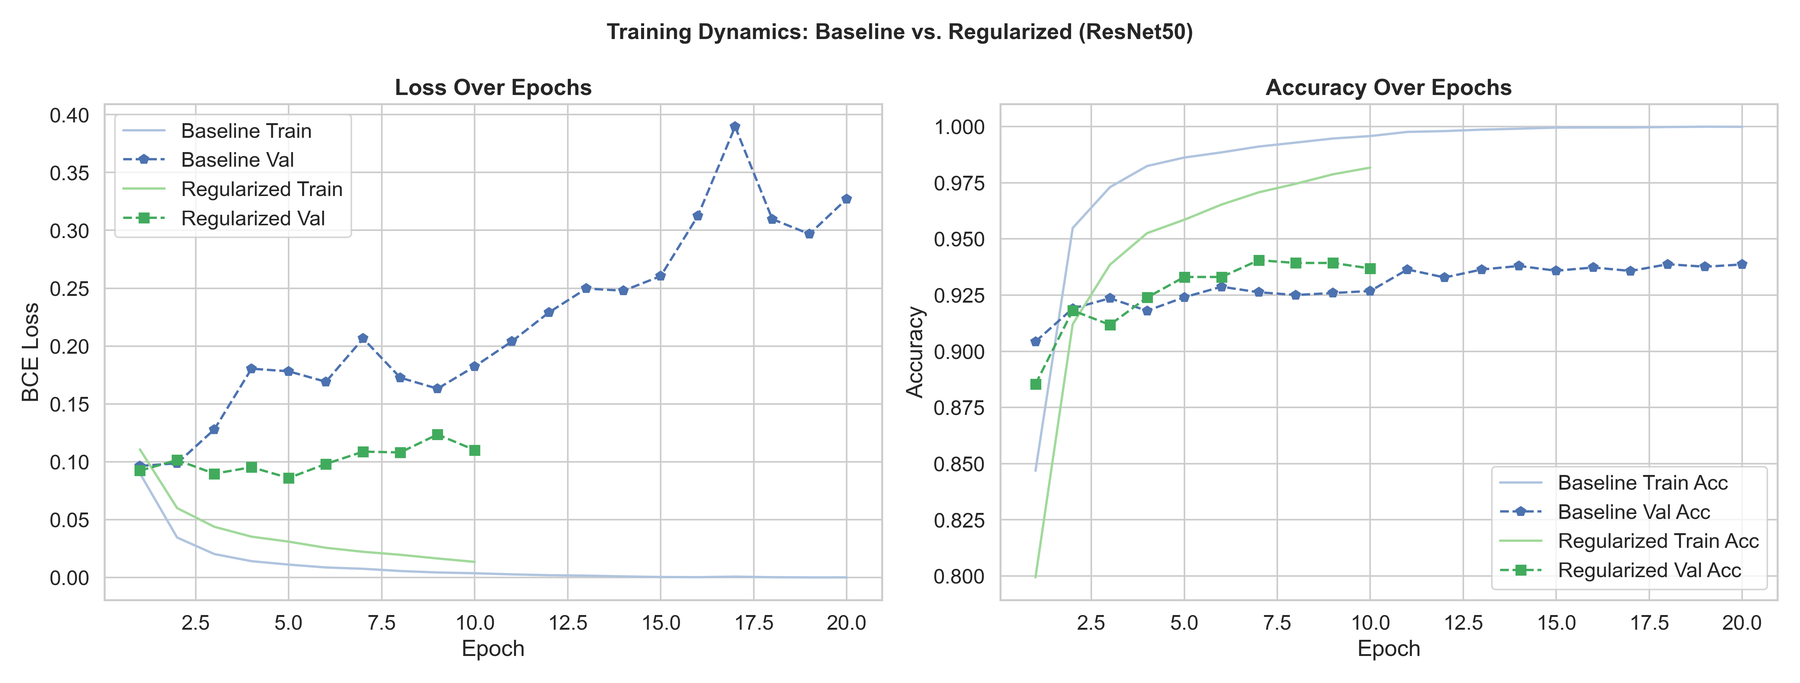
\includegraphics[width=\columnwidth]{images/training_dynamics.png}
\caption{Training and validation loss and validation ROC-AUC trajectories across 20 fine-tuning epochs for ResNet50 Regularized.}
\label{fig:training_dynamics}
\end{figure}

Key findings include:

\textbf{ResNet50 Regularized leads on overall discrimination.} It achieves the highest observed Accuracy ($0.9389$), Recall ($0.9514$), F1 ($0.9633$), ROC-AUC ($0.9718$), PR-AUC ($0.9938$), and MCC ($0.7821$). Residual shortcuts preserve both low-level boundary gradients and semantic facial representations.

\textbf{Xception leads on precision and specificity.} Attaining $\text{Accuracy} = 0.9370$, $\text{F1} = 0.9621$, and the highest precision ($0.9777$), specificity ($0.8830$), and balanced accuracy ($0.9150$), Xception's depthwise separable convolutions effectively decouple spatial and cross-channel color interpolation artifacts.

\textbf{Convolutional models outperform ViT-Small/16.} ViT-Small/16 achieved $\text{Accuracy} = 0.9005$, $\text{F1} = 0.9394$, and $\text{ROC-AUC} = 0.9512$. Localized synthesis artifacts (blending seams, resampling discontinuities) strongly benefit from the local translation equivariance of convolutional filters. Patch tokenization ($16{\times}16$) appears to fragment narrow edge artifacts across patch borders.

\textbf{MobileNetV3-Small offers high throughput with reduced specificity.} Attaining an F1 of 0.9274 at 18.6 FPS on CPU, its lower specificity (70.99\%) reflects the loss of subtle textural features caused by aggressive early channel pruning.

\subsection{Controlled Class-Imbalance Ablation}

Table~\ref{tab:custom_cnn_ablation} summarizes the class-imbalance ablation on the Custom CNN. Without weighting, the model completely collapses to the majority class ($\text{Recall} = 1.0000$, $\text{Specificity} = 0.0000$, $\text{MCC} = 0.0000$), yet exhibits an apparent accuracy of 84.40\% and F1 of 0.9154. Class weighting restores specificity to 74.87\% and MCC to 0.0987, demonstrating the absolute necessity of loss weighting under prevalence skew.

\begin{table}[!t]
\caption{Controlled Class-Imbalance Ablation on Custom CNN.}
\label{tab:custom_cnn_ablation}
\centering
\resizebox{\columnwidth}{!}{%
\begin{tabular}{lcc}
\toprule
\textbf{Metric} & \textbf{Unweighted Baseline} & \textbf{Class-Balanced ($w_{\text{pos}} = 0.1592$)} \\
\midrule
Accuracy & 0.8440 & 0.4324 \\
Precision & 0.8440 & 0.8895 \\
Recall & 1.0000 & 0.3739 \\
Specificity & 0.0000 & 0.7487 \\
F1 Score & 0.9154 & 0.5265 \\
ROC-AUC & 0.5607 & 0.6196 \\
MCC & 0.0000 & 0.0987 \\
\midrule
TP / TN / FP / FN & 8,093 / 0 / 1,496 / 0 & 3,026 / 1,120 / 376 / 5,067 \\
\bottomrule
\end{tabular}%
}
\end{table}

\subsection{Regularization Ablation}

Multi-stage regularization improves all metrics on ResNet50 (Table~\ref{tab:resnet_ablation}). Accuracy increases by $+2.56\%$, Specificity by $+2.07\%$, and MCC improves by $+7.34\%$ ($0.7087 \to 0.7821$), confirming that data augmentation and early stopping prevent late-epoch identity memorization.

\begin{table}[!t]
\caption{Regularization Ablation on ResNet50.}
\label{tab:resnet_ablation}
\centering
\resizebox{\columnwidth}{!}{%
\begin{tabular}{lccc}
\toprule
\textbf{Metric} & \textbf{Baseline} & \textbf{Regularized} & \textbf{$\Delta$} \\
\midrule
Accuracy & 0.9133 & 0.9389 & +2.56\% \\
F1 Score & 0.9474 & 0.9633 & +1.59\% \\
Specificity & 0.8503 & 0.8710 & +2.07\% \\
ROC-AUC & 0.9578 & 0.9718 & +1.40\% \\
MCC & 0.7087 & 0.7821 & +7.34\% \\
\bottomrule
\end{tabular}%
}
\end{table}

\subsection{Bootstrap Confidence Intervals}

Table~\ref{tab:bootstrap_ci} reports crop-level non-parametric bootstrap resampling estimates ($B=1{,}000$, $N=9{,}589$). The 95\% confidence intervals for ResNet50 Regularized (F1: $[0.9603, 0.9663]$) and Xception (F1: $[0.9591, 0.9653]$) overlap across their ranges, establishing that both architectures provide comparable statistical discrimination. Because crop-level resampling treats frames as independent, these intervals represent lower-bound variance estimates compared to video- or component-level cluster bootstrapping.

\begin{table}[!t]
\caption{Non-Parametric Bootstrap Confidence Intervals ($B=1{,}000$, $N=9{,}589$).}
\label{tab:bootstrap_ci}
\centering
\resizebox{\columnwidth}{!}{%
\begin{tabular}{lcccc}
\toprule
\textbf{Architecture} & \textbf{Metric} & \textbf{Mean} & \textbf{SE} & \textbf{95\% CI} \\
\midrule
\multirow{4}{*}{ResNet50 Reg.}
 & Accuracy & 0.9389 & $\pm 0.0025$ & [0.9339, 0.9436] \\
 & F1 Score & 0.9634 & $\pm 0.0015$ & [0.9603, 0.9663] \\
 & ROC-AUC  & 0.9719 & $\pm 0.0021$ & [0.9676, 0.9759] \\
 & PR-AUC   & 0.9939 & $\pm 0.0006$ & [0.9925, 0.9951] \\
\midrule
\multirow{4}{*}{Xception}
 & Accuracy & 0.9371 & $\pm 0.0025$ & [0.9322, 0.9422] \\
 & F1 Score & 0.9621 & $\pm 0.0015$ & [0.9591, 0.9653] \\
 & ROC-AUC  & 0.9707 & $\pm 0.0021$ & [0.9662, 0.9747] \\
 & PR-AUC   & 0.9931 & $\pm 0.0007$ & [0.9917, 0.9944] \\
\bottomrule
\end{tabular}%
}
\end{table}


% ============================================================
% VIII. ERROR ANALYSIS AND DIAGNOSTIC AUDITS
% ============================================================
\section{Error Analysis and Diagnostic Audits}
\label{sec:audits}

\subsection{Per-Manipulation Breakdown}

Table~\ref{tab:manipulation_breakdown} and Fig.~\ref{fig:manipulation_breakdown} break down ResNet50's performance across individual manipulation pipelines.

\begin{table*}[!t]
\caption{Sub-Category Performance Breakdown of ResNet50 Regularized Across Individual Manipulation Pipelines on Held-Out Test Set.}
\label{tab:manipulation_breakdown}
\centering
\begin{tabular*}{\textwidth}{@{\extracolsep{\fill}}lcccccc@{}}
\toprule
\textbf{Category} & \textbf{True Class} & \textbf{$N$} & \textbf{Recall / Spec.} & \textbf{Mean Fake Prob.} & \textbf{Errors} & \textbf{Error Share} \\
\midrule
DeepFakeDetection & FAKE & 615 & \textbf{99.67\%} & 0.9889 & FN\,=\,2 & 0.5\% \\
FaceSwap & FAKE & 1,496 & 97.33\% & 0.9658 & FN\,=\,40 & 10.2\% \\
Deepfakes & FAKE & 1,492 & 97.32\% & 0.9657 & FN\,=\,40 & 10.2\% \\
Face2Face & FAKE & 1,499 & 97.00\% & 0.9622 & FN\,=\,45 & 11.5\% \\
FaceShifter & FAKE & 1,495 & 96.86\% & 0.9568 & FN\,=\,47 & 12.0\% \\
NeuralTextures & FAKE & 1,496 & \textbf{85.36\%} & 0.8363 & FN\,=\,219 & \textbf{55.7\%} \\
\midrule
Original (Authentic) & REAL & 1,496 & \textbf{87.10\%} & 0.1497 & FP\,=\,193 & --- \\
\bottomrule
\end{tabular*}
\end{table*}

\begin{figure}[!t]
\centering
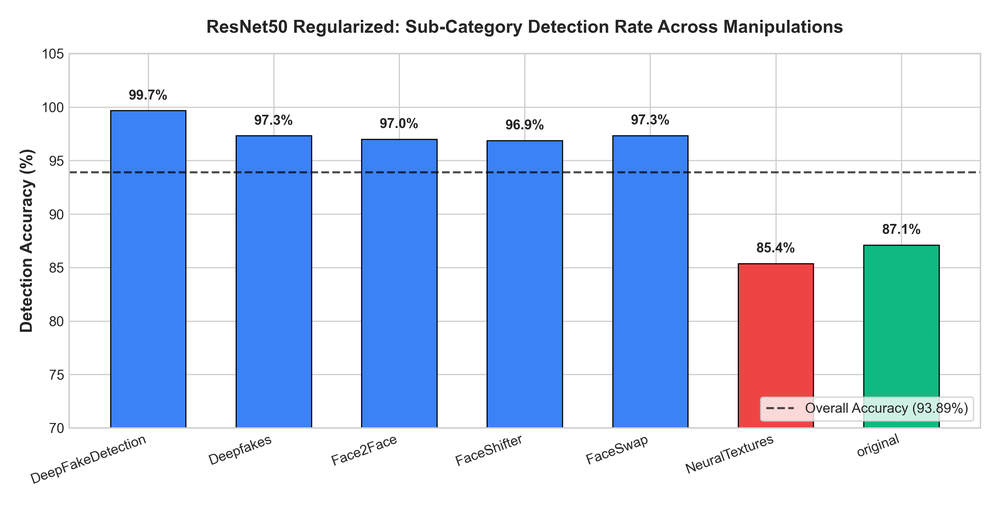
\includegraphics[width=\columnwidth]{images/manipulation_breakdown.png}
\caption{Detection recall and specificity across individual manipulation pipelines in the FaceForensics++ C23 test partition.}
\label{fig:manipulation_breakdown}
\end{figure}

Detection recall exceeded 96\% across five of the six synthesis techniques. However, recall dropped sharply on \textbf{NeuralTextures} to \textbf{85.36\%}. Remarkably, out of 393 total false negatives produced across the entire test set, \textbf{219 (55.7\%)} originated from NeuralTextures alone. Because NeuralTextures restricts deferred neural rendering strictly to the oral cavity, global spatial average pooling dilutes these localized cues across the surrounding authentic face.

\subsection{Confusion Matrix and Confidence Audit}

Fig.~\ref{fig:confusion_matrix} displays the confusion matrix. Across 9,589 samples, ResNet50 produced 586 errors: 193 false positives ($\text{FPR} = 12.90\%$) and 393 false negatives ($\text{FNR} = 4.86\%$).

\begin{figure}[!t]
\centering
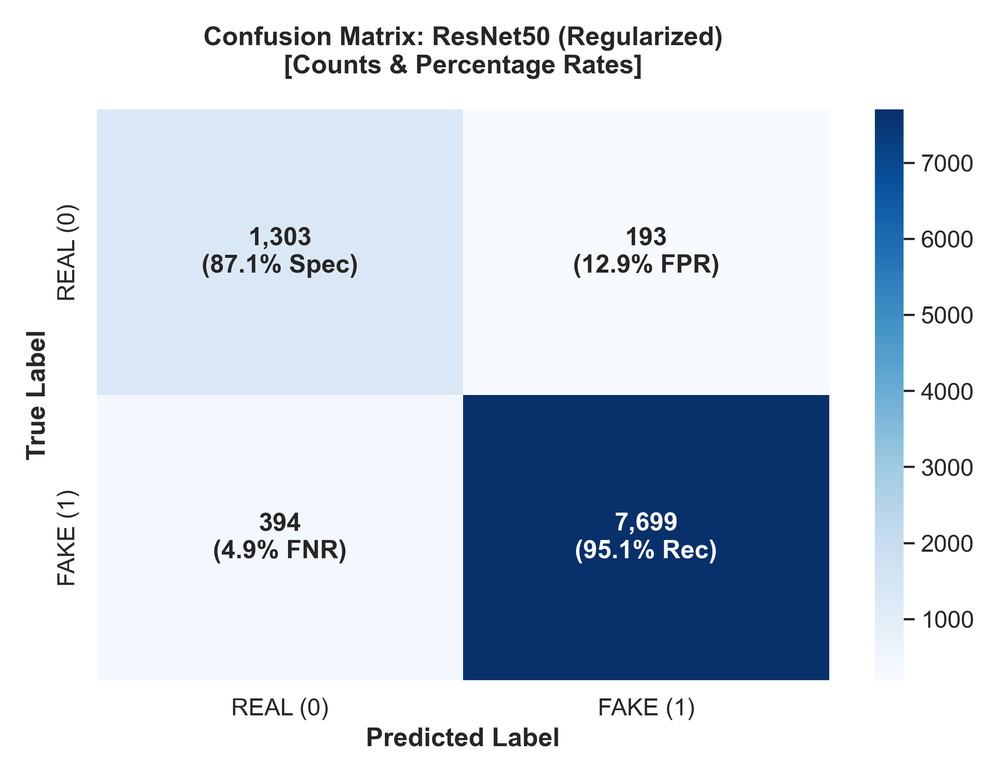
\includegraphics[width=0.85\columnwidth]{images/confusion_matrix.png}
\caption{Confusion matrix of ResNet50 Regularized ($N = 9{,}589$).}
\label{fig:confusion_matrix}
\end{figure}

\begin{figure}[!t]
\centering
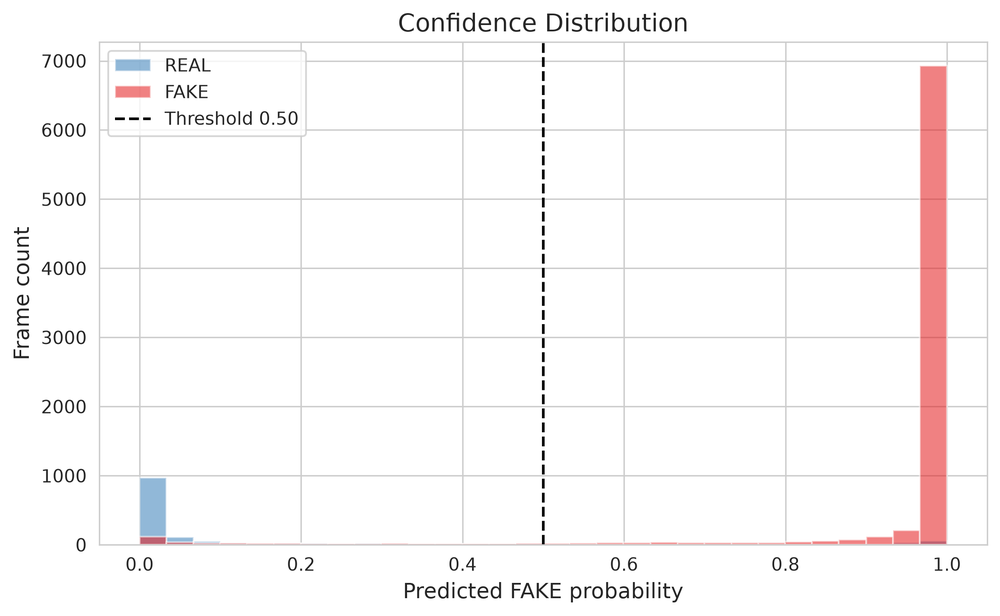
\includegraphics[width=\columnwidth]{images/confidence_distribution.png}
\caption{Predicted probability distribution for authentic real faces (blue) and synthetic fake faces (red).}
\label{fig:confidence_distribution}
\end{figure}

An audit of prediction probabilities (Fig.~\ref{fig:confidence_distribution}) indicates that errors were not confined to the decision boundary: 104 of the 193 false positives exhibited extreme confidence ($\hat{p} > 0.90$), driven by motion blur, harsh directional lighting, and compression blockiness.

\subsection{Probabilistic Calibration Analysis}

ResNet50 Regularized achieved an Expected Calibration Error of $\text{ECE} = 4.07\%$ and Brier score of $0.0499$. Table~\ref{tab:calibration} and Fig.~\ref{fig:calibration_curve} compare the average predicted fake probability against the observed positive-class (FAKE) frequency across 10 uniform bins. Over 90\% of test instances ($8{,}669$ of $9{,}589$) reside in the two extreme bins ($[0.0, 0.1]$ and $[0.9, 1.0]$): the upper bin exhibits a minimal calibration gap ($0.0094$), whereas $[0.0, 0.1]$ shows a gap of $0.1235$ driven by false negatives receiving low fake probabilities. Mid-range bins ($[0.1, 0.7]$) exhibit systematic under-confidence (observed FAKE frequency exceeds predicted probability), an expected consequence of positive-class down-weighting ($w_{\text{pos}} = 0.1592$) shifting raw logits downward.

\begin{table}[!t]
\caption{10-Bin Reliability and Calibration Analysis for ResNet50 Regularized.}
\label{tab:calibration}
\centering
\resizebox{\columnwidth}{!}{%
\begin{tabular}{ccccc}
\toprule
\textbf{Probability Bin} & \textbf{Samples ($|B_m|$)} & \textbf{Mean Pred. $P$} & \textbf{Obs. Fake Freq.} & \textbf{Gap} \\
\midrule
$[0.0, 0.1]$ & 1,314 & 0.0150 & 0.1385 & 0.1235 \\
$[0.1, 0.2]$ & 129 & 0.1463 & 0.5194 & 0.3730 \\
$[0.2, 0.3]$ & 94 & 0.2505 & 0.4681 & 0.2176 \\
$[0.3, 0.4]$ & 76 & 0.3461 & 0.6579 & 0.3118 \\
$[0.4, 0.5]$ & 83 & 0.4553 & 0.6024 & 0.1471 \\
$[0.5, 0.6]$ & 92 & 0.5527 & 0.7935 & 0.2408 \\
$[0.6, 0.7]$ & 116 & 0.6494 & 0.8362 & 0.1868 \\
$[0.7, 0.8]$ & 130 & 0.7505 & 0.7692 & 0.0187 \\
$[0.8, 0.9]$ & 200 & 0.8570 & 0.8950 & 0.0380 \\
$[0.9, 1.0]$ & 7,355 & 0.9953 & 0.9859 & 0.0094 \\
\bottomrule
\end{tabular}%
}
\end{table}

\begin{figure}[!t]
\centering
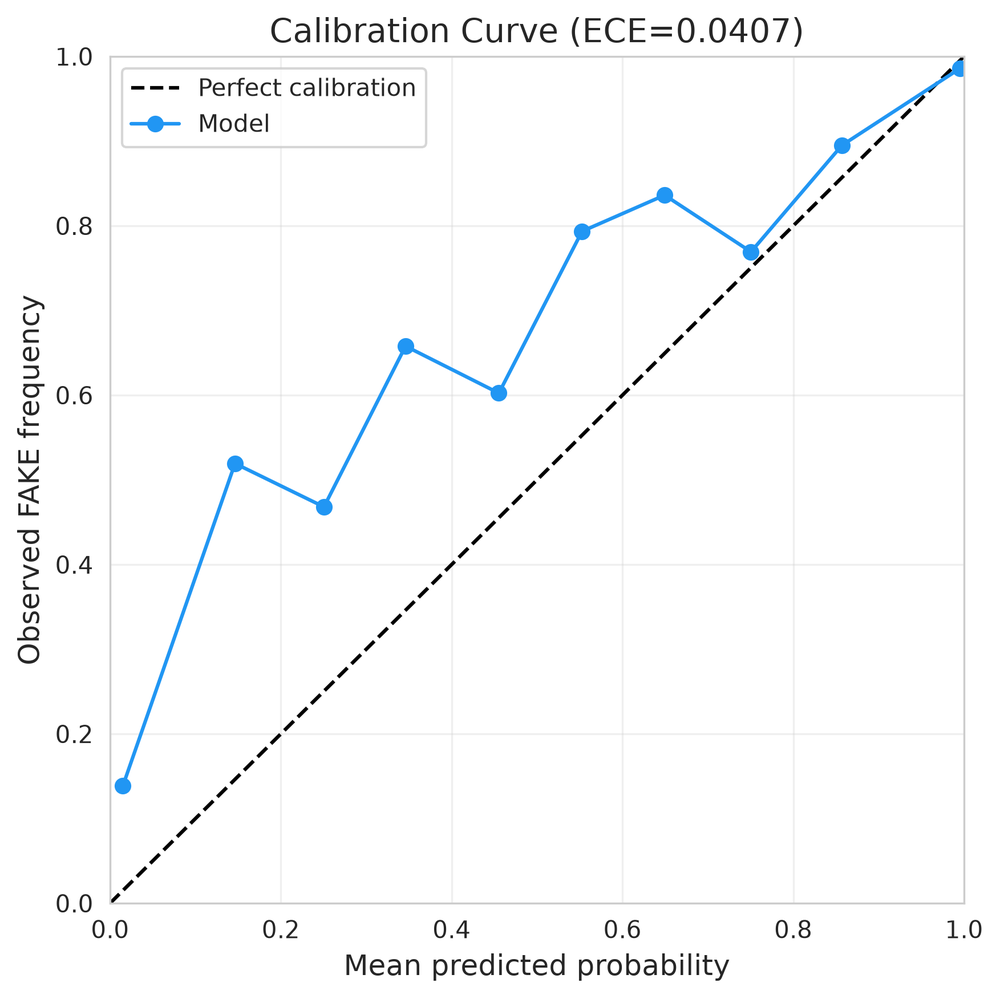
\includegraphics[width=0.85\columnwidth,height=2.3in,keepaspectratio]{images/calibration_curve.png}
\caption{Reliability diagram and calibration curve for ResNet50 Regularized ($\text{ECE} = 4.07\%$).}
\label{fig:calibration_curve}
\end{figure}

\subsection{Perturbation Robustness and Compression Cliff}

Table~\ref{tab:robustness} and Fig.~\ref{fig:robustness_curve} summarize robustness across eight perturbation conditions on an $N=502$ synthetic subset. The model exhibits strong stability under moderate spatial perturbations (100\% recall under Gaussian blur, 99.4\% under noise, and 100\% under downscale-upscale cycles). In contrast, JPEG compression reveals a sharp performance cliff: recall sits at 94.82\% at Q=90 and 96.41\% at Q=70 (reflecting single-run finite-sample variability on the 502-image subset), then drops abruptly to 72.51\% at Q=50 and collapses to 39.64\% at Q=30, marking the threshold where quantization eliminates discriminative high-frequency gradients.

\begin{table}[!t]
\caption{Perturbation Stress-Testing on Synthetic Image Subset ($N=502$).}
\label{tab:robustness}
\centering
\resizebox{\columnwidth}{!}{%
\begin{tabular}{lcccc}
\toprule
\textbf{Perturbation Condition} & \textbf{$N$} & \textbf{Recall (\%)} & \textbf{Mean Fake Prob.} & \textbf{Retention (\%)} \\
\midrule
Clean Baseline & 502 & \textbf{98.21\%} & 0.9699 & 100.0\% \\
JPEG Quality 90 & 502 & 94.82\% & 0.9289 & 96.5\% \\
JPEG Quality 70 & 502 & 96.41\% & 0.9384 & 98.2\% \\
JPEG Quality 50 & 502 & 72.51\% & 0.7135 & 73.8\% \\
JPEG Quality 30 & 502 & \textbf{39.64\%} & 0.4029 & \textbf{40.4\%} \\
Gaussian Blur ($r = 1.5$) & 502 & 100.00\% & 0.9992 & 101.8\% \\
Gaussian Noise ($\sigma = 0.05$) & 502 & 99.40\% & 0.9685 & 101.2\% \\
Downscale 4$\times$ + Upscale & 502 & 100.00\% & 0.9955 & 101.8\% \\
\bottomrule
\end{tabular}%
}
\end{table}

\begin{figure}[!t]
\centering
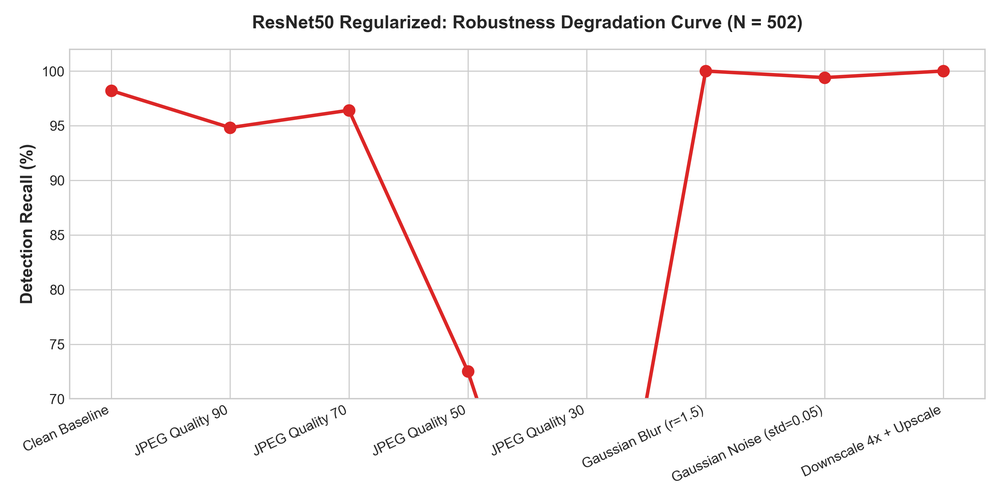
\includegraphics[width=\columnwidth,height=2.0in,keepaspectratio]{images/robustness_curve.png}
\caption{Performance retention across compression sweeps and spatial image perturbations ($N=502$).}
\label{fig:robustness_curve}
\end{figure}


% ============================================================
% IX. VISUAL EXPLAINABILITY
% ============================================================
\section{Visual Explainability via Grad-CAM}
\label{sec:explainability}

\begin{figure*}[!t]
\centering
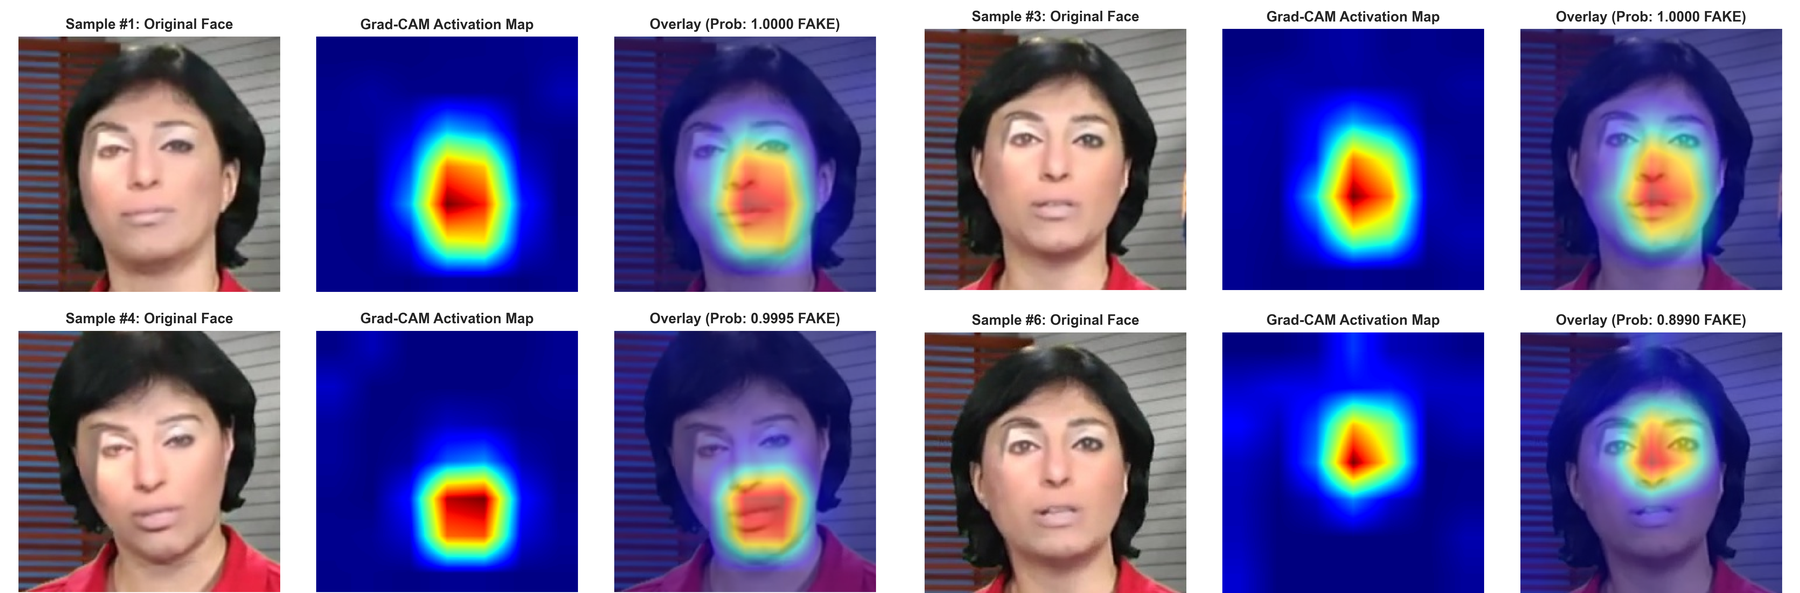
\includegraphics[width=\textwidth,height=2.35in,keepaspectratio]{images/gradcam_sample_grid.png}
\caption{Grad-CAM spatial activation maps for ResNet50 Regularized at the final residual block. Heatmaps show that attention concentrates on facial boundaries (for face-swap methods) and perioral regions (for reenactment methods). Background regions receive minimal activation.}
\label{fig:gradcam_sample_grid}
\end{figure*}

We extract Gradient-weighted Class Activation Mapping (Grad-CAM) \cite{selvaraju2017gradcam} at ResNet50's final residual block (\texttt{layer4[-1]}) to inspect spatial decision regions (Fig.~\ref{fig:gradcam_sample_grid}). For identity replacement algorithms (Deepfakes, FaceSwap), activation heatmaps concentrate along the jawline, chin contours, and facial boundaries where Poisson blending stitches donor and target skin textures. For reenactment techniques (Face2Face, NeuralTextures), saliency shifts predominantly to the oral cavity, lips, and perioral transitions.

While these visualizations indicate alignment with physical manipulation boundaries, we emphasize that post-hoc saliency maps provide qualitative diagnostic visualization rather than definitive causal verification of model mechanics. Saliency heatmaps must be interpreted as supporting qualitative evidence rather than proof of out-of-distribution robustness.


% ============================================================
% X. COMPUTATIONAL EFFICIENCY
% ============================================================
\section{Computational Efficiency}
\label{sec:complexity}

Table~\ref{tab:efficiency} and Fig.~\ref{fig:efficiency_comparison} summarize computational latency and parameter footprints measured under CPU-only execution (12th Gen Intel Core i5-12500H, 16 GB RAM, Windows 11, Python 3.13.3, PyTorch 2.8.0+cpu) with batch size 1, 10 warm-up iterations, and 100 timed forward passes (\texttt{time.perf\_counter()}), excluding image preprocessing. MobileNetV3-Small provides the fastest pre-trained throughput (18.6 FPS, 53.9 ms latency) with a 17.6 MB checkpoint, suitable for lightweight screening. ResNet50 achieves leading accuracy at 93.5 ms (10.7 FPS), whereas Xception incurs substantially higher CPU latency (1,372.0 ms, 0.7 FPS) due to unoptimized depthwise separable convolutions on CPU. ViT-Small/16 achieves 13.5 FPS (73.9 ms) but lags behind convolutional backbones in discriminative accuracy.

\begin{table}[!t]
\caption{Inference Latency, Throughput, and Checkpoint Footprint on Standard CPU.}
\label{tab:efficiency}
\centering
\resizebox{\columnwidth}{!}{%
\begin{tabular}{lcccc}
\toprule
\textbf{Architecture} & \textbf{Params} & \textbf{Checkpoint} & \textbf{CPU Latency} & \textbf{Throughput} \\
\midrule
Custom CNN & 93,825 & 1.1 MB & 13.25 $\pm$ 1.28 ms & 75.5 FPS \\
MobileNetV3-Small & 1,518,881 & 17.6 MB & 53.89 $\pm$ 10.27 ms & 18.6 FPS \\
ViT-Small/16 & 21,666,049 & 248.1 MB & 73.87 $\pm$ 10.89 ms & 13.5 FPS \\
ResNet50 & 23,510,081 & 269.5 MB & 93.52 $\pm$ 7.64 ms & 10.7 FPS \\
EfficientNet-B0 & 4,008,829 & 46.4 MB & 116.86 $\pm$ 107.49 ms & 8.6 FPS \\
Xception & 20,809,001 & 238.6 MB & 1371.96 $\pm$ 778.59 ms & 0.7 FPS \\
\bottomrule
\end{tabular}%
}
\end{table}

\begin{figure}[!t]
\centering
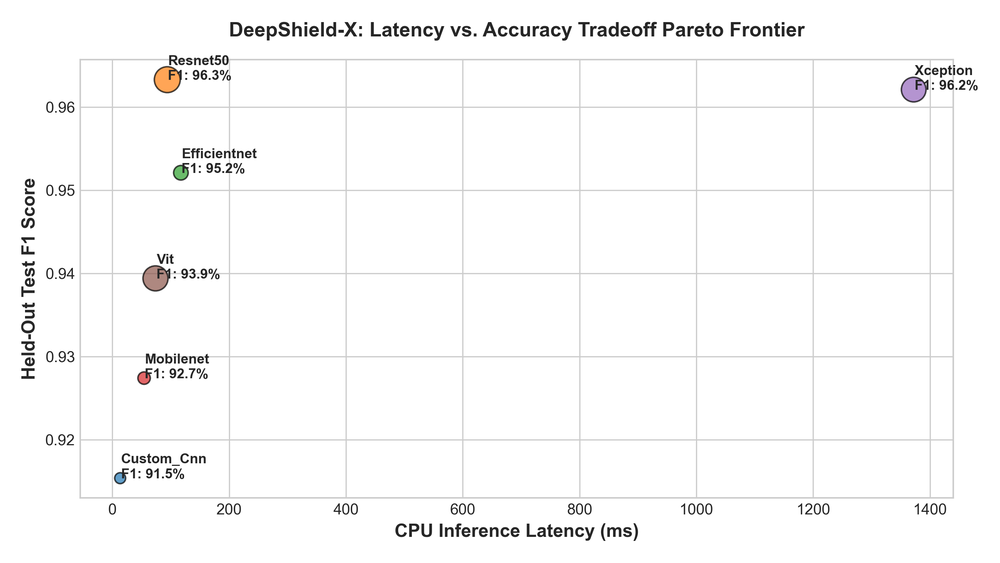
\includegraphics[width=\columnwidth,height=2.2in,keepaspectratio]{images/efficiency_comparison.png}
\caption{Inference latency versus F1 score trade-off across evaluated architectures.}
\label{fig:efficiency_comparison}
\end{figure}


% ============================================================
% XI. DISCUSSION
% ============================================================
\section{Discussion}
\label{sec:discussion}

\textbf{Identity-disjoint splitting matters.} By assigning graph connected components atomically, the evaluation protocol ensures that test metrics reflect genuine artifact detection rather than actor recognition. As established by Dong et al.\ \cite{dong2023implicit}, leakage between splits can artificially inflate accuracy by over 10 percentage points, making identity-disjoint partitioning the most vital methodological prerequisite in forensic benchmarking.

\textbf{Accuracy is dangerously misleading.} The unweighted Custom CNN ablation (84.40\% accuracy, 0.00\% specificity) demonstrates that standard accuracy is structurally incapable of assessing performance under benchmark class skew. Balanced metrics such as MCC \cite{chicco2020advantages} must be mandatory in multimedia forensic evaluations.

\textbf{Convolutional models outperform transformers on compressed media.} In our controlled benchmark, ResNet50 and Xception consistently surpassed ViT-Small/16. Manipulation artifacts (blending seams, color interpolation discontinuities) are high-frequency local phenomena. Convolutional filters, with built-in translation equivariance and local inductive bias, are naturally equipped to capture these subtle spatial cues. Fixed patch tokenization ($16 \times 16$) in standard ViTs may fragment continuous boundary artifacts across adjacent patches, confirming findings from unified benchmarks \cite{yan2023deepfakebench} and hybrid architectures \cite{coccomini2022crossefficientvit}.

\textbf{NeuralTextures represents a structural blind spot.} Accounting for 55.7\% of all false negatives, NeuralTextures poses a unique challenge because its modifications are confined strictly to the oral cavity. Global average pooling aggregates features across the entire spatial grid, effectively drowning out subtle localized mouth artifacts within a vast authentic background. This confirms the necessity of localized attention mechanisms \cite{zhao2021multiattentional} and dedicated perioral temporal models \cite{haliassos2021lips}.

\textbf{The compression cliff is real.} The sharp collapse in recall below JPEG Q=50 underscores the forensic reliance on high-frequency spatial gradients, showing that aggressive quantization on social platforms degrades spatial detector efficacy.


% ============================================================
% XII. LIMITATIONS
% ============================================================
\section{Limitations}
\label{sec:limitations}

\begin{enumerate}
    \item \textbf{Single benchmark scope.} Experiments were conducted on FaceForensics++ C23; cross-dataset evaluation on external wild corpora was not performed.
    \item \textbf{Frame-level modeling.} The framework operates on static crops without exploiting inter-frame temporal or optical flow consistency \cite{haliassos2021lips}.
    \item \textbf{Perturbation subset scale.} Stress-testing was conducted on an $N=502$ synthetic image subset.
    \item \textbf{Absence of adaptive adversarial attacks.} Evaluations assessed digital perturbations but did not test gradient-based adversarial manipulations.
    \item \textbf{Generative paradigm coverage.} Media consisted of autoencoder and morphable model fakes; diffusion-synthesized manipulations remain unmeasured.
    \item \textbf{Post-hoc explainability.} Grad-CAM is a qualitative diagnostic tool and does not provide formal causal guarantees.
    \item \textbf{Crop-level bootstrap vs. cluster testing.} Confidence intervals use crop-level resampling rather than video- or component-level cluster bootstrapping, and do not replace paired hypothesis testing.
    \item \textbf{Metadata-level identity graph.} Union-Find isolates all source-target pairings encoded in dataset filenames, but does not cluster unrelated YouTube clips via biometric face embeddings.
\end{enumerate}


% ============================================================
% XIII. CONCLUSION
% ============================================================
\section{Conclusion}
\label{sec:conclusion}

This paper presented an experimental investigation of deepfake detection on FaceForensics++ C23 under an empirically verified identity-disjoint protocol. By formulating sequence partitioning via graph union-find, we eliminated identity leakage across 69,273 face crops. Our controlled experiments demonstrated that unweighted loss functions induce majority-class collapse, masking total failure on real faces behind an 84.40\% accuracy score.

Among six evaluated architectures, ResNet50 Regularized and Xception achieved leading performance (F1 = 0.9633 and 0.9621), outperforming Vision Transformers on compressed media. Sub-category audits revealed NeuralTextures as the primary failure mode (55.7\% of all false negatives), and perturbation testing revealed a compression cliff below JPEG Q=50. Future work will investigate cross-dataset generalization, spatio-temporal dynamics, and localized oral cavity attention to counter subtle reenactment forgeries.

\FloatBarrier

\section*{Acknowledgment}
The author thanks the faculty advisors and peers in the Department of Computer Science and Engineering for their guidance and feedback throughout this research.

\bibliographystyle{IEEEtran}
\bibliography{references}

\end{document}
